% ASSERT_CONVENTION: natural_units=natural, metric_signature=mostly_minus, fourier_convention=physics, coupling_convention=alpha_s, generator_normalization=T(fund)=1/2, covariant_derivative_sign=D_mu=partial_mu-igA
%
% Lecture 1: Anomaly matching and the conformal window
% Part of: The Dualised Standard Model -- Part III Lecture Notes
%
\documentclass[11pt,a4paper]{article}
% ASSERT_CONVENTION: natural_units=natural, metric_signature=mostly_minus, fourier_convention=physics, coupling_convention=alpha_s, generator_normalization=T(fund)=1/2, covariant_derivative_sign=D_mu=partial_mu-igA
%
% CONVENTIONS (Seiberg hep-th/9411149)
% Metric: (+,-,-,-) (mostly minus)
% T(fund) = 1/2 per Weyl fermion
% b_0 = (11N_c - 2N_f)/3 for N_f Dirac flavours
% D_mu = partial_mu - ig A_mu^a T^a
% A(fund) = 1 (cubic anomaly coefficient per fundamental Weyl fermion)
% alpha_s = g_s^2 / (4 pi)
% R[Q] = (N_f - N_c)/N_f; R[W] = 2
% N_f counts Dirac flavour pairs (each = 2 Weyl fermions)
%
% This file is \input{} by all lecture files.

%% ---------- Document class ----------
% (loaded by the wrapper; preamble only provides packages and macros)

%% ---------- Standard packages ----------
\usepackage{amsmath,amssymb,amsthm,mathtools}
\usepackage{hyperref}
\usepackage[capitalise,noabbrev]{cleveref}
\usepackage{enumitem}
\usepackage{booktabs}
\usepackage{array}
\usepackage{xcolor}
\usepackage{tikz}
\usetikzlibrary{arrows.meta,decorations.markings,positioning,calc}
\usepackage{fancybox}
\usepackage{tcolorbox}
\tcbuselibrary{skins,breakable}
\usepackage{slashed}              % Feynman slash notation
\usepackage{cite}                 % compressed citation lists

%% ---------- Hyperref configuration ----------
\hypersetup{
  colorlinks=true,
  linkcolor=blue!70!black,
  citecolor=green!50!black,
  urlcolor=blue!80!black,
  pdfauthor={Part III Lecture Notes},
  pdftitle={The Dualised Standard Model}
}

%% ---------- Theorem environments ----------
\theoremstyle{plain}
\newtheorem{theorem}{Theorem}[section]
\newtheorem{lemma}[theorem]{Lemma}
\newtheorem{proposition}[theorem]{Proposition}
\newtheorem{corollary}[theorem]{Corollary}

\theoremstyle{definition}
\newtheorem{definition}[theorem]{Definition}
\newtheorem{example}[theorem]{Example}
\newtheorem{exercise}{Exercise}[section]

\theoremstyle{remark}
\newtheorem{remark}[theorem]{Remark}

%% ---------- Physics macros: gauge groups and representations ----------
\newcommand{\Nc}{N_{\!c}}
\newcommand{\Nf}{N_{\!f}}
\newcommand{\SU}[1]{\mathrm{SU}(#1)}
\newcommand{\UU}[1]{\mathrm{U}(#1)}

% Representations
\newcommand{\fund}{\square}
\newcommand{\antifund}{\overline{\square}}
\newcommand{\adj}{\mathrm{adj}}
\newcommand{\antisym}{\wedge^{\!2}}        % antisymmetric rank-2
\newcommand{\sym}{\mathrm{S}_2}           % symmetric rank-2

%% ---------- Physics macros: group theory constants ----------
% Dynkin index: Tr(T^a T^b) = T(R) delta^{ab}
\newcommand{\Tfund}{\tfrac{1}{2}}          % T(fund) = 1/2 per Weyl fermion
\newcommand{\Tadj}{\Nc}                    % T(adj) = N_c
\newcommand{\Cfund}{\frac{\Nc^2 - 1}{2\Nc}}  % C_2(fund)
\newcommand{\Cadj}{\Nc}                    % C_2(adj)

% Cubic anomaly coefficient: A(R) = Tr_R[T^a {T^b, T^c}] with A(fund) = 1
\newcommand{\Afund}{1}

%% ---------- Physics macros: beta function ----------
\newcommand{\bzero}{b_0}
\newcommand{\bone}{b_1}
\newcommand{\alphas}{\alpha_s}
\newcommand{\gs}{g_s}

%% ---------- Physics macros: SUSY / R-charge ----------
\newcommand{\Rcharge}[1]{R[#1]}
\newcommand{\Wsup}{W}                      % superpotential

%% ---------- Physics macros: covariant derivative and field strength ----------
\newcommand{\Dmu}{D_\mu}
\newcommand{\Fmn}{F_{\mu\nu}}
\newcommand{\Ftilde}{\widetilde{F}_{\mu\nu}}

%% ---------- Physics macros: common abbreviations ----------
\newcommand{\ie}{\textit{i.e.}}
\newcommand{\eg}{\textit{e.g.}}
\newcommand{\cf}{\textit{cf.}}
\newcommand{\IR}{\ensuremath{\mathrm{IR}}}
\newcommand{\UV}{\ensuremath{\mathrm{UV}}}
\newcommand{\AF}{\ensuremath{\mathrm{AF}}}
\newcommand{\BZ}{\ensuremath{\mathrm{BZ}}}
\newcommand{\NSVZ}{\ensuremath{\mathrm{NSVZ}}}
\newcommand{\SQCD}{\ensuremath{\mathrm{SQCD}}}
\newcommand{\QCD}{\ensuremath{\mathrm{QCD}}}
\newcommand{\SM}{\ensuremath{\mathrm{SM}}}
\newcommand{\Tr}{\mathrm{Tr}}

%% ---------- Convention box macro ----------
\newtcolorbox{conventionbox}[1][]{%
  enhanced,
  colback=blue!5!white,
  colframe=blue!60!black,
  fonttitle=\bfseries,
  title={Conventions},
  #1
}

%% ---------- Comparison table style ----------
\newtcolorbox{comparisontable}[1][]{%
  enhanced,
  colback=orange!5!white,
  colframe=orange!70!black,
  fonttitle=\bfseries,
  title={Comparison},
  #1
}

%% ---------- Warning / important box ----------
\newtcolorbox{warningbox}[1][]{%
  enhanced,
  colback=red!5!white,
  colframe=red!70!black,
  fonttitle=\bfseries,
  title={Important},
  #1
}

%% ---------- Preview / forward-reference box ----------
\newtcolorbox{previewbox}[1][]{%
  enhanced,
  colback=green!5!white,
  colframe=green!50!black,
  fonttitle=\bfseries,
  title={Preview},
  #1
}

%% ---------- Page layout ----------
\usepackage[margin=2.5cm]{geometry}
\setlength{\parskip}{0.4em}
\setlength{\parindent}{0em}

%% ---------- Section formatting ----------
\usepackage{titlesec}
\titleformat{\section}{\Large\bfseries}{\thesection}{1em}{}
\titleformat{\subsection}{\large\bfseries}{\thesubsection}{1em}{}

%% ---------- End of preamble ----------


\title{\textbf{Lecture 1: Anomaly Matching and the Conformal Window}}
\author{The Dualised Standard Model --- Part III Lecture Notes}
\date{Lent Term 2027}

\begin{document}
\maketitle

\tableofcontents
\newpage

%% ========================================================================
%%  SECTION 1: Introduction and overview
%% ========================================================================
\section{Introduction and overview}
\label{sec:intro}

These lecture notes develop the idea that the Standard Model of particle
physics might be understood as a \emph{magnetic dual} theory---the
low-energy, weakly-coupled description of a more fundamental, strongly-coupled
\emph{electric} theory at high energies.  The programme, due primarily to
Sannino and collaborators \cite{Sannino2024}, builds on Seiberg's
electric--magnetic duality for supersymmetric gauge theories
\cite{Seiberg1995} and extends it, with appropriate caveats, to
non-supersymmetric gauge theories.

\textbf{Prerequisites.}  We assume the Michaelmas QFT course: gauge theory
(classical and quantised), anomalies (ABJ anomaly, triangle diagrams), and
the representation theory of $\SU{\Nc}$ at the level of Peskin and
Schroeder~\cite{PS1995}.  \emph{No knowledge of supersymmetry is required}
for this lecture; SUSY will be introduced from scratch in Lecture~2.

\textbf{Course goal.}  By the end of these notes, students will be able to:
\begin{enumerate}[label=(\roman*)]
  \item construct the dualised Standard Model from a Pati--Salam-like
    electric theory with only fermions and no elementary scalars;
  \item verify anomaly matching between the electric and magnetic
    descriptions for the full SM gauge group
    $\SU{3}_c \times \SU{2}_L \times \UU{1}_Y$;
  \item derive parametric expressions for the SM fermion mass hierarchy,
    the Fermi scale $v \approx 246\;\mathrm{GeV}$, and the QCD scale
    $\Lambda_{\QCD} \approx 200\;\mathrm{MeV}$ from the dual theory.
\end{enumerate}

\textbf{Outline of Lecture~1.}  We begin with the mathematical tools that
underpin all subsequent lectures: 't~Hooft anomaly matching and the
conformal window of gauge theories.  Specifically:
\begin{itemize}
  \item \S\ref{sec:conventions}: conventions and notation.
  \item \S\ref{sec:gauge-anomaly}: review of gauge anomaly cancellation (recap from Michaelmas).
  \item \S\ref{sec:thooft}: 't~Hooft anomaly matching for global symmetries.
  \item \S\ref{sec:warmup}: worked example---$\SU{3}$ QCD with $\Nf = 2$.
  \item \S\ref{sec:general-anomaly}: general anomaly matching for $\SU{\Nc}$ with $\Nf$ flavours.
  \item \S\ref{sec:conformal}: the beta function and the conformal window.
  \item \S\ref{sec:summary}: summary and preview of Lecture~2.
\end{itemize}

\begin{remark}[Chan--Tsou disambiguation]
\label{rem:chantsou}
The term ``Dualised Standard Model'' has been used in a \emph{different}
sense by Chan and Tsou \cite{ChanTsou1999,Tsou2001}.  Their programme
applies a loop-space \emph{Hodge duality} within the SM gauge group
$\SU{3}_c \times \SU{2}_L \times \UU{1}_Y$ itself, identifying dual
colour as a generation symmetry.  This is conceptually and technically
distinct from the Seiberg-type \emph{electric--magnetic duality between
different theories} pursued by Sannino and collaborators.  Throughout
these notes, ``dualised Standard Model'' always refers to the
Cacciapaglia--Sannino gauge-fermion duality programme
\cite{Sannino2024}, not the Chan--Tsou construction.%
\footnote{For the Chan--Tsou programme, see \cite{ChanTsou1999} and the
  lecture notes \cite{Tsou2001}.  Their construction has no direct
  connection to Seiberg duality or the anomaly matching machinery
  developed in these lectures.}
\end{remark}


%% ========================================================================
%%  SECTION 2: Convention table
%% ========================================================================
\section{Conventions and notation}
\label{sec:conventions}

All conventions follow Seiberg \cite{Seiberg1995} unless otherwise noted.

\begin{conventionbox}[title={Conventions for these lecture notes}]
\renewcommand{\arraystretch}{1.3}
\begin{tabular}{@{}l l l@{}}
\toprule
\textbf{Quantity} & \textbf{Convention} & \textbf{Comment} \\
\midrule
Units & $\hbar = c = 1$ (natural) & \\
Metric & $\eta_{\mu\nu} = \mathrm{diag}(+1,-1,-1,-1)$ & mostly minus \\
Dynkin index & $\Tr(T^a T^b) = \Tfund\, \delta^{ab}$ & fundamental of $\SU{\Nc}$ \\
Covariant derivative & $\Dmu = \partial_\mu - i\gs A_\mu^a T^a$ & \\
Anomaly coefficient & $A(\fund) = 1$ & cubic; per fundamental Weyl fermion \\
Beta function & $\bzero = \dfrac{11\Nc - 2\Nf}{3}$ & $\Nf$ Dirac flavours \\
$\Nf$ counting & $\Nf$ = number of Dirac pairs & each pair = 2 Weyl fermions \\
Coupling & $\alphas = \gs^2/(4\pi)$ & \\
$R$-charge (SUSY) & $\Rcharge{Q} = (\Nf - \Nc)/\Nf$ & non-anomalous $R$-symmetry \\
\bottomrule
\end{tabular}
\end{conventionbox}

\begin{warningbox}[title={Weyl vs.\ Dirac counting}]
  Throughout these notes, $\Nf$ counts the number of \textbf{Dirac flavour
  pairs}.  Each Dirac fermion consists of two Weyl fermions (one
  left-handed, one right-handed).  In the SUSY literature, one often
  encounters $\Nf$ chiral superfield \emph{pairs} $(Q_i,\,\widetilde{Q}_i)$,
  $i = 1,\ldots,\Nf$---each such pair corresponds to one Dirac flavour and
  contains \emph{two} Weyl fermions.  Some references use $T(\fund) = 1$
  per \emph{Dirac} fermion; we use $T(\fund) = \Tfund$ per \emph{Weyl}
  fermion (equivalently, per fundamental of $\SU{\Nc}$).  The two
  conventions differ by a factor of~2 that propagates to all anomaly
  coefficients and the conformal window boundaries.
\end{warningbox}

\textbf{Group theory data.}  We collect the Dynkin indices and quadratic
Casimirs for common representations of $\SU{\Nc}$:

\begin{center}
\renewcommand{\arraystretch}{1.3}
\begin{tabular}{@{}l c c c@{}}
\toprule
\textbf{Representation} $R$ & \textbf{Dimension} $d(R)$
  & \textbf{Dynkin index} $T(R)$ & \textbf{Quadratic Casimir} $C_2(R)$ \\
\midrule
Fundamental $\Nc$ & $\Nc$ & $\Tfund$ & $\Cfund$ \\[3pt]
Antifundamental $\overline{\Nc}$ & $\Nc$ & $\Tfund$ & $\Cfund$ \\[3pt]
Adjoint & $\Nc^2 - 1$ & $\Nc$ & $\Nc$ \\[3pt]
Antisymmetric $\wedge^2$ & $\frac{\Nc(\Nc-1)}{2}$ & $\frac{\Nc-2}{2}$
  & $\frac{(\Nc-1)(\Nc+2)}{2\Nc}$ \\[3pt]
Symmetric $\mathrm{S}_2$ & $\frac{\Nc(\Nc+1)}{2}$ & $\frac{\Nc+2}{2}$
  & $\frac{(\Nc-1)(\Nc+4)}{2\Nc}$ \\[3pt]
\bottomrule
\end{tabular}
\end{center}

\noindent\textit{Check:} For $\SU{3}$, the fundamental has
$C_2(\fund) = (9-1)/6 = 4/3$.  This is the standard QCD result.

The \textbf{cubic anomaly coefficient} is defined by
\begin{equation}
  A(R)\, d^{abc} = \Tr_R\!\bigl[T^a \{T^b, T^c\}\bigr],
  \label{eq:anomaly-coeff-def}
\end{equation}
where $d^{abc}$ is the totally symmetric $d$-symbol of $\SU{\Nc}$,
normalised so that $A(\fund) = 1$.

\begin{center}
\renewcommand{\arraystretch}{1.3}
\begin{tabular}{@{}l c@{}}
\toprule
\textbf{Representation} & $A(R)$ \\
\midrule
Fundamental $\Nc$ & $+1$ \\
Antifundamental $\overline{\Nc}$ & $-1$ \\
Adjoint & $2\Nc$ \\
Antisymmetric $\wedge^2$ & $\Nc - 4$ \\
Symmetric $\mathrm{S}_2$ & $\Nc + 4$ \\
\bottomrule
\end{tabular}
\end{center}

\noindent Note that $A(\overline{R}) = -A(R)$, and that
$A(\adj) = 0$ for $\SU{2}$ (since $\SU{2}$ has no cubic anomaly:
all representations are (pseudo-)real).


%% ========================================================================
%%  SECTION 3: Gauge anomaly cancellation (review)
%% ========================================================================
\section{Review: gauge anomaly cancellation}
\label{sec:gauge-anomaly}

We begin with a brief review of material from the Michaelmas QFT course.
The purpose is to set up the contrast with 't~Hooft anomaly matching
in~\S\ref{sec:thooft}.

\subsection{The ABJ anomaly}

Consider a triangle Feynman diagram with three external gauge bosons
coupled to a chiral fermion in representation~$R$ of the gauge group.
The one-loop amplitude contains an \emph{anomaly}: the classical symmetry
$\partial_\mu j^\mu_5 = 0$ is violated at the quantum level,
\begin{equation}
  \partial_\mu j^\mu_5 = \frac{1}{16\pi^2}\, \Fmn^a \widetilde{F}^{a\,\mu\nu},
  \label{eq:abj}
\end{equation}
where $\widetilde{F}^{a\,\mu\nu} = \tfrac{1}{2}\epsilon^{\mu\nu\rho\sigma}
F^a_{\rho\sigma}$.  This is the Adler--Bell--Jackiw (ABJ) anomaly
\cite{Adler1969,BellJackiw1969}.

\subsection{Gauge anomaly cancellation: the consistency requirement}

For a gauge theory to be \emph{quantum mechanically consistent}, all gauge
anomalies must vanish.  This means that for every triple of gauge
generators $(T^a, T^b, T^c)$, the anomaly coefficient
\begin{equation}
  \mathcal{A}^{abc}_{\text{gauge}}
  = \sum_{\text{Weyl fermions}\; i}
    \Tr\!\bigl[T^a_{R_i}\{T^b_{R_i}, T^c_{R_i}\}\bigr]
  \label{eq:gauge-anomaly}
\end{equation}
must \emph{vanish}: $\mathcal{A}^{abc}_{\text{gauge}} = 0$.  The sum runs
over all left-handed Weyl fermions in the theory (with right-handed Weyl
fermions contributing with a minus sign, since $\overline{R}$ has
$A(\overline{R}) = -A(R)$).

\subsection{Example: the Standard Model}

In the Standard Model, gauge anomaly cancellation is a non-trivial constraint
on the fermion content.  For a single generation, the fermion representations
under $\SU{3}_c \times \SU{2}_L \times \UU{1}_Y$ are:
\begin{center}
\renewcommand{\arraystretch}{1.3}
\begin{tabular}{@{}l c c c c@{}}
\toprule
\textbf{Field} & $\SU{3}_c$ & $\SU{2}_L$ & $Y$ & Chirality \\
\midrule
$Q_L = (u_L,\, d_L)$ & $\mathbf{3}$ & $\mathbf{2}$ & $+1/6$ & L \\
$u_R$ & $\mathbf{3}$ & $\mathbf{1}$ & $+2/3$ & R \\
$d_R$ & $\mathbf{3}$ & $\mathbf{1}$ & $-1/3$ & R \\
$L_L = (\nu_L,\, e_L)$ & $\mathbf{1}$ & $\mathbf{2}$ & $-1/2$ & L \\
$e_R$ & $\mathbf{1}$ & $\mathbf{1}$ & $-1$ & R \\
\bottomrule
\end{tabular}
\end{center}

We state without rederivation that all gauge anomalies cancel.
For instance:
\begin{itemize}
  \item $\SU{3}_c^2 \,\UU{1}_Y$: contributions from $Q_L$, $u_R$, $d_R$
    cancel:
    $2 \times \Tfund \times (+\tfrac{1}{6})
     - 1 \times \Tfund \times (+\tfrac{2}{3})
     - 1 \times \Tfund \times (-\tfrac{1}{3})
     = \Tfund(+\tfrac{1}{3} - \tfrac{2}{3} + \tfrac{1}{3}) = 0$.
  \item $\UU{1}_Y^3$: sum of $Y^3$ over all left-handed Weyl fermions
    (converting right-handed to left-handed with a sign flip in $Y$)
    vanishes.
\end{itemize}

\textbf{Key point:} Gauge anomaly cancellation is a \emph{consistency
requirement}.  If it fails, the theory is inconsistent at the quantum level.
We now contrast this with a very different use of anomalies.


%% ========================================================================
%%  SECTION 4: 't Hooft anomaly matching
%% ========================================================================
\section{'t~Hooft anomaly matching}
\label{sec:thooft}

\subsection{Gauge anomaly cancellation vs.\ 't~Hooft anomaly matching}

The following distinction is \textbf{critical} and is a source of widespread
confusion (see \eg\ Peskin \cite{PeskinTASI1996}, Sec.~3).

\begin{comparisontable}[title={Gauge anomaly cancellation vs.\ 't~Hooft anomaly matching}]
\renewcommand{\arraystretch}{1.4}
\begin{tabular}{@{}p{3.5cm} p{5cm} p{5cm}@{}}
\toprule
& \textbf{Gauge anomaly cancellation} & \textbf{'t~Hooft anomaly matching} \\
\midrule
\textbf{Symmetry type}
  & \emph{Gauged} symmetry
  & \emph{Global} symmetry \\[4pt]
\textbf{Condition}
  & Anomaly must \textbf{vanish} (= 0)
  & Anomaly must \textbf{match} (\UV{} = \IR) \\[4pt]
\textbf{Physical meaning}
  & Quantum consistency of the gauge theory
  & Constraint on the \IR{} spectrum \\[4pt]
\textbf{What if violated?}
  & Theory is \textbf{inconsistent}
  & Proposed \IR{} spectrum is \textbf{wrong} \\[4pt]
\textbf{Role of RG flow}
  & Holds at every scale
  & Relates two different scales (\UV{} and \IR) \\[4pt]
\textbf{Computational object}
  & $\sum_i \Tr[T^a_{R_i}\{T^b_{R_i}, T^c_{R_i}\}] = 0$
  & $\sum_{\UV} \Tr[T^a\{T^b, T^c\}] = \sum_{\IR} \Tr[T^a\{T^b, T^c\}]$ \\
\bottomrule
\end{tabular}
\end{comparisontable}

\noindent The triangle diagrams and the group-theoretic computation are
\emph{identical}---both involve $\Tr[T^a\{T^b, T^c\}]$.  But the
\emph{generators} are different (gauged vs.\ global), and the
\emph{interpretation} is different (vanishing vs.\ matching).  Never confuse
the two.

\subsection{Statement of the result}

\begin{theorem}['t~Hooft anomaly matching \cite{tHooft1980}]
\label{thm:anomaly-matching}
Let $G_{\text{gauge}}$ be the gauge group of an asymptotically free gauge
theory, and let $G_{\text{global}}$ be its exact global symmetry group.
For every triple of generators $(T^a, T^b, T^c)$ of $G_{\text{global}}$
(and/or gravity), the anomaly coefficient
\begin{equation}
  \mathcal{A}^{abc}
  = \sum_{\text{massless fermions}}
    \Tr\!\bigl[T^a\{T^b, T^c\}\bigr]
  \label{eq:anomaly-matching}
\end{equation}
takes the \textbf{same value} when computed using the \UV{} degrees of
freedom (quarks, gluons, \ldots) and when computed using the \IR{} degrees
of freedom (hadrons, Goldstone bosons, \ldots):
\begin{equation}
  \boxed{\mathcal{A}^{abc}_{\UV} = \mathcal{A}^{abc}_{\IR}.}
  \label{eq:matching-boxed}
\end{equation}
\end{theorem}

\noindent This is an \emph{exact} result: by the Adler--Bardeen theorem
\cite{AdlerBardeen1969}, the anomaly coefficient~\eqref{eq:anomaly-coeff-def}
receives contributions only at one loop and is not renormalised by
higher-order corrections.  Therefore the anomaly computed at any scale
is the same, and in particular the \UV{} and \IR{} values must agree.

\subsection{The spectator argument}
\label{subsec:spectator}

We now present 't~Hooft's elegant proof via spectator fields
\cite{tHooft1980,PeskinTASI1996}.  The argument proceeds in five steps:

\begin{enumerate}[label=\textbf{Step \arabic*:}, leftmargin=3.5em]
  \item \textbf{Promote the global symmetry to a gauge symmetry.}
    Take the global symmetry $G_{\text{global}}$ and weakly gauge it:
    introduce gauge bosons $B_\mu^a$ for $G_{\text{global}}$ with a very
    small coupling $g_{\text{w}} \to 0$.  (This is a thought experiment;
    $g_{\text{w}}$ is an auxiliary parameter that will be sent to zero at the
    end.)

  \item \textbf{Add spectator fermions to cancel the new gauge anomaly.}
    The original fermions will generically produce a non-vanishing
    $G_{\text{global}}^3$ gauge anomaly (since we have now gauged what was
    previously a global symmetry).  Add \emph{spectator fermions}---free
    fermions that are \emph{singlets} under the original gauge group
    $G_{\text{gauge}}$ but carry charges under the newly gauged
    $G_{\text{global}}$---chosen so that the total gauge anomaly of the
    combined system vanishes.  This is always possible by appropriate choice
    of spectator representations.

  \item \textbf{The combined theory is consistent at all scales.}
    Since the total $G_{\text{global}}^3$ gauge anomaly now vanishes, the
    combined theory (original fermions $+$ spectators, with both
    $G_{\text{gauge}}$ and $G_{\text{global}}$ gauged) is a consistent
    quantum theory at all energy scales.

  \item \textbf{Spectators are free and unchanged by RG flow.}
    The spectator fermions are singlets under $G_{\text{gauge}}$ and
    interact only via the $G_{\text{global}}$ gauge bosons at coupling
    $g_{\text{w}} \to 0$.  Therefore they are free fields: they do not
    participate in the strong dynamics of $G_{\text{gauge}}$, and their
    anomaly contribution is the \emph{same} in the \UV{} and in the \IR.

  \item \textbf{Anomaly matching follows.}
    The total anomaly is zero at all scales.  The spectator contribution is
    the same at all scales.  Therefore the anomaly from the \emph{original}
    fermions must also be the same at all scales:
    \[
      \underbrace{\mathcal{A}_{\text{original}}^{\UV}}_{\text{quarks}}
      \;+\;
      \underbrace{\mathcal{A}_{\text{spectators}}}_{\text{unchanged}}
      \;=\;
      0
      \;=\;
      \underbrace{\mathcal{A}_{\text{original}}^{\IR}}_{\text{hadrons}}
      \;+\;
      \underbrace{\mathcal{A}_{\text{spectators}}}_{\text{unchanged}},
    \]
    hence $\mathcal{A}_{\text{original}}^{\UV}
    = \mathcal{A}_{\text{original}}^{\IR}$. \qed
\end{enumerate}

\subsection{Important caveats}

\begin{enumerate}[label=(\alph*)]
  \item \textbf{Anomaly matching is necessary but not sufficient.}
    Matching the anomaly coefficients constrains the \IR{} spectrum but does
    \emph{not} uniquely determine it.  There may be multiple
    anomaly-consistent proposals for the \IR{} content; additional physical
    input (dynamics, lattice evidence, SUSY, \ldots) is needed to select
    among them.

  \item \textbf{Only exact global symmetries participate.}
    Anomaly matching applies to global symmetries that are \emph{exact}---not
    explicitly or spontaneously broken.  Spontaneously broken symmetries are
    still exact symmetries of the Lagrangian and \emph{do} participate in
    anomaly matching (the Goldstone bosons are massless and must be counted
    in the \IR{} spectrum).  However, \emph{anomalous} symmetries---those
    broken by quantum effects, such as $\UU{1}_A$ in QCD---must \emph{not}
    be included.

  \item \textbf{The result is exact.}
    By the Adler--Bardeen theorem \cite{AdlerBardeen1969}, the anomaly
    is one-loop exact.  There are no higher-order corrections, no
    non-perturbative corrections, and no scheme dependence.  This is
    what makes anomaly matching such a powerful tool in strongly coupled
    gauge theories, where perturbation theory fails.
\end{enumerate}


%% ========================================================================
%%  SECTION 5: Warm-up example: SU(3) QCD with Nf = 2
%% ========================================================================
\section{Warm-up: \texorpdfstring{$\SU{3}$}{SU(3)} QCD with \texorpdfstring{$\Nf = 2$}{Nf=2}}
\label{sec:warmup}

We now illustrate anomaly matching with a concrete and familiar example:
QCD with two light flavours.

\subsection{UV spectrum}

The \UV{} theory is $\SU{3}$ gauge theory with $\Nf = 2$ massless Dirac
quarks---the $u$ and $d$ quarks.  In terms of Weyl fermions:
\begin{itemize}
  \item $q_{L,i}^{\,\alpha}$: left-handed quarks,
    $\alpha = 1,2,3$ (colour), $i = 1,2$ (flavour).
    Representation: $(\mathbf{3}, \mathbf{2}, 1)$ under
    $\SU{3}_c \times \SU{2}_L \times \SU{2}_R$.
  \item $q_{R,i}^{\,\alpha}$: right-handed quarks (equivalently,
    left-handed antiquarks $\bar{q}_{L,i\,\alpha}$).
    Representation: $(\overline{\mathbf{3}}, 1, \mathbf{2})$ under
    $\SU{3}_c \times \SU{2}_L \times \SU{2}_R$.
\end{itemize}

The \emph{exact global symmetry} (for massless quarks) is
$\SU{2}_L \times \SU{2}_R \times \UU{1}_B$, where $\UU{1}_B$ is baryon
number with $B[q] = 1/3$.

\begin{warningbox}[title={$\UU{1}_A$ is anomalous}]
  The axial symmetry $\UU{1}_A$ is explicitly broken by the ABJ anomaly
  \eqref{eq:abj}.  It is \emph{not} an exact global symmetry and must
  \textbf{not} be included in the anomaly matching conditions.
\end{warningbox}

\subsection{UV anomaly coefficients}

Let us compute the $\SU{2}_L^3$ anomaly.  The only fermions charged under
$\SU{2}_L$ are the left-handed quarks $q_{L,i}^{\,\alpha}$, which form
$\Nc = 3$ copies (one per colour) of the fundamental of $\SU{2}_L$.  Each
copy contributes $A(\fund_{\SU{2}}) = 1$ to the cubic anomaly.  Therefore:
\begin{equation}
  \mathcal{A}_{\UV}\bigl[\SU{2}_L^3\bigr]
  = \Nc \times A(\fund_{\SU{2}})
  = 3 \times 1 = 3.
  \label{eq:uv-anomaly-su2L}
\end{equation}
By an identical argument (exchanging $L \leftrightarrow R$),
$\mathcal{A}_{\UV}[\SU{2}_R^3] = 3$.

\subsection{IR spectrum: confinement and chiral symmetry breaking}

At low energies, $\SU{3}_c$ confines and chiral symmetry breaks
spontaneously:
\[
  \SU{2}_L \times \SU{2}_R \;\xrightarrow{\;\langle\bar{q}q\rangle \neq 0\;}\;
  \SU{2}_V \quad (\text{isospin}).
\]

The low-energy degrees of freedom are:
\begin{itemize}
  \item \textbf{3 Goldstone bosons} (pions):
    $\pi^+$, $\pi^-$, $\pi^0$, in the adjoint (= triplet) of $\SU{2}_V$.
    These are $(\mathbf{3}, \mathbf{3})_0$ under $\SU{2}_L \times \SU{2}_R$
    in a non-linear sigma model representation.
    Goldstone bosons are \emph{scalars} and do not contribute to the
    anomaly coefficient $\mathcal{A}^{abc}$ (which involves only fermions
    in perturbation theory).

  \item \textbf{Baryons} (proton and neutron):
    $p$ and $n$, forming an isospin doublet.  As composite fermions made of
    three quarks, the baryons are in $(\mathbf{2}, \mathbf{1})$ under
    $\SU{2}_L \times \SU{2}_R$ after chiral symmetry breaking---more
    precisely, in $(\mathbf{2}, \mathbf{1}) \oplus (\mathbf{1}, \mathbf{2})$
    as Dirac fermions.  The left-handed component transforms as $\mathbf{2}$
    under $\SU{2}_L$; the right-handed component is a singlet under $\SU{2}_L$.
\end{itemize}

\subsection{IR anomaly matching}

For $\SU{2}_L^3$, the only \IR{} fermions contributing are the left-handed
baryons in the $\mathbf{2}$ of $\SU{2}_L$:
\begin{equation}
  \mathcal{A}_{\IR}\bigl[\SU{2}_L^3\bigr]
  = 1 \times A(\fund_{\SU{2}}) = 1.
  \label{eq:ir-anomaly-wrong}
\end{equation}

But $\mathcal{A}_{\UV} = 3 \neq 1 = \mathcal{A}_{\IR}$!  Does anomaly
matching fail?

\textbf{Resolution.}  The analysis above is incomplete.  The Goldstone
bosons do not contribute to perturbative anomalies, but they \emph{do}
contribute to anomaly matching through the
\emph{Wess--Zumino--Witten (WZW) term} in the chiral Lagrangian
\cite{WessZumino1971,Witten1983}.  The WZW term is a topological term
that encodes the anomaly of the underlying microscopic (quark) theory
in the effective low-energy (pion) theory.  Its coefficient is fixed by
anomaly matching to be exactly $\Nc = 3$.

Including the WZW contribution:
\begin{equation}
  \mathcal{A}_{\IR}\bigl[\SU{2}_L^3\bigr]
  = \underbrace{1}_{\text{baryons}}
  + \underbrace{2}_{\text{WZW term}}
  = 3
  = \mathcal{A}_{\UV}\bigl[\SU{2}_L^3\bigr].
  \label{eq:ir-anomaly-matched}
\end{equation}

\begin{remark}
  This example illustrates a subtle but important point: in theories with
  spontaneous chiral symmetry breaking, the Goldstone bosons \emph{do}
  carry anomaly information through the WZW term.  The coefficient of the
  WZW term is \emph{not} a free parameter---it is fixed by anomaly matching
  and equals $\Nc$.  This is a powerful consistency check on the chiral
  Lagrangian description of QCD.
\end{remark}

\begin{remark}
  An alternative perspective (following 't~Hooft's original analysis
  \cite{tHooft1980}) considers the scenario where chiral symmetry is
  \emph{not} broken.  In that case, the IR spectrum must contain massless
  composite fermions whose anomaly coefficients match those of the quarks.
  This ``confinement without chiral symmetry breaking'' scenario requires
  very specific baryon representations and is believed not to occur for
  $\SU{3}$ with $\Nf = 2$.  The point is that anomaly matching
  \emph{constrains} the possible IR dynamics: \emph{either} chiral symmetry
  breaks (producing Goldstones with a WZW term) \emph{or} massless
  composite fermions must appear.  This is a non-trivial constraint that
  rules out certain confinement scenarios.
\end{remark}


%% ========================================================================
%%  SECTION 6: General anomaly matching for SU(Nc) with Nf flavours
%% ========================================================================
\section{General anomaly matching for \texorpdfstring{$\SU{\Nc}$}{SU(Nc)}
  with \texorpdfstring{$\Nf$}{Nf} flavours}
\label{sec:general-anomaly}

We now set up the anomaly matching conditions for the general case that
will be used throughout these lectures: $\SU{\Nc}$ gauge theory with
$\Nf$ Dirac flavours in the fundamental representation.

\subsection{Global symmetry}
\label{subsec:global-sym}

The massless theory has the global symmetry
\begin{equation}
  G_{\text{global}}
  = \SU{\Nf}_L \times \SU{\Nf}_R \times \UU{1}_B \times \UU{1}_A.
  \label{eq:global-sym}
\end{equation}

However, $\UU{1}_A$ is anomalous (the ABJ anomaly) and is broken to a
discrete subgroup $\mathbb{Z}_{2\Nf}$.  The $\UU{1}_A$ anomaly is
\emph{not} matched---it is a genuine breaking of the symmetry, not a
constraint.

\begin{warningbox}[title={Do not match the anomalous $\UU{1}_A$}]
  The axial $\UU{1}_A$ symmetry is broken by the ABJ anomaly and must
  \textbf{not} be included in the 't~Hooft anomaly matching conditions.
  Only the non-anomalous symmetries participate in matching.
\end{warningbox}

The \textbf{exact} global symmetry group for anomaly matching purposes is
\begin{equation}
  G_{\text{exact}}
  = \SU{\Nf}_L \times \SU{\Nf}_R \times \UU{1}_B.
  \label{eq:exact-global-sym}
\end{equation}

The baryon number assignments follow the Seiberg convention
\cite{Seiberg1995}:
\begin{equation}
  B[Q_i] = \frac{1}{\Nc}, \qquad
  B[\widetilde{Q}^i] = -\frac{1}{\Nc},
  \label{eq:baryon-number}
\end{equation}
where $Q_i$ ($i = 1,\ldots,\Nf$) are left-handed Weyl fermions in the
fundamental of $\SU{\Nc}$, and $\widetilde{Q}^i$ are left-handed Weyl
fermions in the antifundamental.  A baryon $B \sim Q^{\Nc}$ then has
$B[B] = 1$.

\subsection{UV anomaly coefficients}

The \UV{} degrees of freedom are $\Nc \Nf$ left-handed Weyl fermions $Q_i^\alpha$
in the $(\fund, \fund_L, \mathbf{1}_R)$ of $\SU{\Nc} \times \SU{\Nf}_L \times \SU{\Nf}_R$
and $\Nc \Nf$ left-handed Weyl fermions $\widetilde{Q}^{i\,\alpha}$ in the
$(\antifund, \mathbf{1}_L, \fund_R)$.

The independent anomaly coefficients to match are:

\begin{enumerate}[label=(\arabic*)]
  \item \textbf{$\SU{\Nf}_L^3$:}
    Only $Q_i^\alpha$ contributes.
    There are $\Nc$ copies (one per colour) of the fundamental of $\SU{\Nf}_L$.
    \begin{equation}
      \mathcal{A}_{\UV}\bigl[\SU{\Nf}_L^3\bigr]
      = \Nc \times A(\fund_{\SU{\Nf}}) = \Nc.
      \label{eq:uv-sunfL3}
    \end{equation}

  \item \textbf{$\SU{\Nf}_R^3$:}
    By $L \leftrightarrow R$ symmetry,
    \begin{equation}
      \mathcal{A}_{\UV}\bigl[\SU{\Nf}_R^3\bigr] = \Nc.
      \label{eq:uv-sunfR3}
    \end{equation}

  \item \textbf{$\SU{\Nf}_L^2 \,\UU{1}_B$:}
    This is a mixed anomaly.  The $Q_i^\alpha$ contribute with
    $\UU{1}_B$ charge $B = 1/\Nc$, and there are $\Nc$ colours:
    \begin{equation}
      \mathcal{A}_{\UV}\bigl[\SU{\Nf}_L^2\,\UU{1}_B\bigr]
      = \Nc \times T(\fund_{\SU{\Nf}}) \times \frac{1}{\Nc}
      = \frac{1}{2}.
      \label{eq:uv-sunfL2-u1b}
    \end{equation}
    (Using $T(\fund) = 1/2$.)

  \item \textbf{$\SU{\Nf}_R^2 \,\UU{1}_B$:}
    The $\widetilde{Q}^i$ have $B = -1/\Nc$ and contribute similarly:
    \begin{equation}
      \mathcal{A}_{\UV}\bigl[\SU{\Nf}_R^2\,\UU{1}_B\bigr]
      = \Nc \times T(\fund_{\SU{\Nf}}) \times \Bigl(-\frac{1}{\Nc}\Bigr)
      = -\frac{1}{2}.
      \label{eq:uv-sunfR2-u1b}
    \end{equation}

  \item \textbf{$\UU{1}_B^3$:}
    The $Q$ fields contribute $\Nc \Nf$ Weyl fermions with $B = 1/\Nc$;
    the $\widetilde{Q}$ fields contribute $\Nc \Nf$ Weyl fermions with
    $B = -1/\Nc$:
    \begin{equation}
      \mathcal{A}_{\UV}\bigl[\UU{1}_B^3\bigr]
      = \Nc\Nf \times \Bigl(\frac{1}{\Nc}\Bigr)^{\!3}
      + \Nc\Nf \times \Bigl(-\frac{1}{\Nc}\Bigr)^{\!3}
      = 0.
      \label{eq:uv-u1b3}
    \end{equation}

  \item \textbf{$\UU{1}_B$ (gravitational):}
    The gravitational anomaly is proportional to $\sum_i B_i$:
    \begin{equation}
      \mathcal{A}_{\UV}\bigl[\UU{1}_B\text{-grav}\bigr]
      = \Nc\Nf \times \frac{1}{\Nc}
      + \Nc\Nf \times \Bigl(-\frac{1}{\Nc}\Bigr)
      = 0.
      \label{eq:uv-u1b-grav}
    \end{equation}
\end{enumerate}

\noindent Collecting the results:

\begin{center}
\renewcommand{\arraystretch}{1.3}
\begin{tabular}{@{}l c l@{}}
\toprule
\textbf{Anomaly triple} & $\mathcal{A}_{\UV}$ & \textbf{Comment} \\
\midrule
$\SU{\Nf}_L^3$ & $\Nc$ & $\Nc$ colours in fundamental of $\SU{\Nf}_L$ \\
$\SU{\Nf}_R^3$ & $\Nc$ & by $L \leftrightarrow R$ \\
$\SU{\Nf}_L^2\,\UU{1}_B$ & $\frac{1}{2}$ & uses $T(\fund) = \frac{1}{2}$,
  $B = 1/\Nc$ \\
$\SU{\Nf}_R^2\,\UU{1}_B$ & $-\frac{1}{2}$ & uses $B[\widetilde{Q}] = -1/\Nc$ \\
$\UU{1}_B^3$ & $0$ & $Q$ and $\widetilde{Q}$ cancel \\
$\UU{1}_B\text{-grav}$ & $0$ & $Q$ and $\widetilde{Q}$ cancel \\
\bottomrule
\end{tabular}
\end{center}

These six anomaly coefficients must be matched by \emph{any} proposed
\IR{} spectrum.  They will be our primary tool for verifying Seiberg
duality in Lecture~3.

\begin{exercise}
  Verify the entries in the table above by explicit computation.  In
  particular, check that the $\SU{\Nf}_L^2\,\UU{1}_B$ anomaly gives
  $1/2$ (not $1$ or $\Nc$) by carefully tracking the Dynkin index
  $T(\fund) = 1/2$ and the baryon number normalisation $B = 1/\Nc$.
  \textit{(Exercise Set~1, Problem~1.)}
\end{exercise}


%% ========================================================================
%%  SECTION 7: Beta function and conformal window
%% ========================================================================
\section{The beta function and the conformal window}
\label{sec:conformal}

We now turn to the second key ingredient for these lectures: the
\emph{conformal window}---the range of $\Nf$ for which an $\SU{\Nc}$ gauge
theory with fundamental matter flows to a non-trivial IR fixed point rather
than confining.

\subsection{One-loop beta function}

The running of the gauge coupling is governed by the beta function.  At
one loop:
\begin{equation}
  \mu\frac{d\alphas}{d\mu}
  = -\frac{\bzero}{2\pi}\,\alphas^2 + \mathcal{O}(\alphas^3),
  \label{eq:beta-1loop}
\end{equation}
where the one-loop coefficient is
\begin{equation}
  \boxed{%
  \bzero = \frac{11\Nc - 2\Nf}{3}
  }
  \qquad (\Nf \text{ Dirac flavours in the fundamental}).
  \label{eq:b0}
\end{equation}

\textbf{Derivation sketch} (not rederived here; see \cite{PS1995}, Ch.~16).
The coefficient $\bzero$ receives two competing contributions:
\begin{itemize}
  \item \textbf{Gluon self-coupling (antiscreening):} $+\frac{11}{3}\,T(\adj) \times 2
    = \frac{11}{3}\,\Nc$.
    The non-Abelian gauge field self-interactions produce an
    \emph{antiscreening} effect that makes the coupling decrease at short
    distances.  This is the origin of asymptotic freedom.
  \item \textbf{Fermion loops (screening):} $-\frac{4}{3}\,T(\fund) \times \Nf
    = -\frac{4}{3} \times \frac{1}{2} \times \Nf = -\frac{2\Nf}{3}$.
    Each Dirac fermion contributes $2$ Weyl fermions, each with
    $T(\fund) = 1/2$, giving $T_{\text{Dirac}} = 1$.
    Fermion loops produce a conventional screening effect.
\end{itemize}

\noindent Combining: $\bzero = \frac{11\Nc}{3} - \frac{2\Nf}{3}
= \frac{11\Nc - 2\Nf}{3}$.

\textbf{Asymptotic freedom} requires $\bzero > 0$, \ie,
\begin{equation}
  \Nf < \frac{11\Nc}{2}.
  \label{eq:af-bound}
\end{equation}
For $\SU{3}$: $\Nf < 16.5$, so $\Nf \leq 16$ preserves asymptotic freedom
and $\Nf \geq 17$ loses it.

\textit{Check:} $\SU{3}$, $\Nf = 6$ (physical QCD): $\bzero = (33 - 12)/3 = 7 > 0$.
QCD is asymptotically free.  $\checkmark$

\subsection{Two-loop beta function and the Banks--Zaks fixed point}

At two loops, the beta function acquires a second coefficient $\bone$:
\begin{equation}
  \mu\frac{d\alphas}{d\mu}
  = -\frac{\bzero}{2\pi}\,\alphas^2
  - \frac{\bone}{4\pi^2}\,\alphas^3
  + \mathcal{O}(\alphas^4),
  \label{eq:beta-2loop}
\end{equation}
where
\begin{equation}
  \bone = \frac{1}{3}\Bigl[34\Nc^2 - \Nf\Bigl(13\Nc - \frac{3}{\Nc}\Bigr)\Bigr].
  \label{eq:b1}
\end{equation}

The beta function has a non-trivial zero (besides $\alphas = 0$) when
$\bzero > 0$ and $\bone < 0$.  Setting $\beta(\alphas^*) = 0$ at two loops:
\begin{equation}
  \alphas^*
  = -\frac{\bzero}{\bone}\,\frac{2\pi}{1}
  = -\frac{2\pi\,\bzero}{\bone}.
  \label{eq:bz-fixedpoint}
\end{equation}
For this to be a physical (positive) fixed point, we need $\bone < 0$
(since $\bzero > 0$).

This is the \textbf{Banks--Zaks fixed point} \cite{BanksZaks1982}: when
$\Nf$ is just below $11\Nc/2$, so that $\bzero$ is small and positive while
$\bone$ is negative, the coupling runs from $\alphas = 0$ in the \UV{} to a
small, perturbatively calculable value $\alphas^*$ in the \IR.  The theory
flows to a \emph{conformal field theory} (CFT) in the infrared.

\textit{Check:} For $\SU{3}$, $\Nf = 16$:
$\bzero = (33 - 32)/3 = 1/3$,
$\bone = (34 \times 9 - 16 \times (39 - 1))/3 = (306 - 608)/3 = -302/3 < 0$.
So $\alphas^* = -2\pi \times (1/3)/(-302/3) = 2\pi/302 \approx 0.021 \ll 1$.
The fixed point is perturbatively reliable.  $\checkmark$

\subsection{The conformal window}

The \textbf{conformal window} is the range of $\Nf$ for which the
$\SU{\Nc}$ gauge theory is asymptotically free but flows to a non-trivial
\IR{} fixed point (an interacting CFT) rather than confining.

\begin{itemize}
  \item \textbf{Upper boundary:} $\Nf = 11\Nc/2$ (loss of asymptotic freedom).
    Above this value, $\bzero < 0$ and the theory is \IR{} free (trivial).
  \item \textbf{Lower boundary (non-SUSY):} The lower boundary is where
    confinement and chiral symmetry breaking set in.  This is
    \emph{not} perturbatively calculable and is \textbf{debated}.
    Two-loop estimates give $\Nf^* \sim 8$--$12$ for $\SU{3}$, but these
    are unreliable near the lower boundary where $\alphas^*$ is no longer
    small.  Lattice simulations \cite{DeGrand2015,Hasenbusch2021} and
    functional RG methods give somewhat different values.
\end{itemize}

\begin{warningbox}[title={The non-SUSY lower boundary is model-dependent}]
  The two-loop estimate of the conformal window lower boundary is only
  a rough guide.  Different methods (ladder approximation, functional RG,
  lattice Monte Carlo) give different values for $\Nf^*$.
  The \emph{upper} boundary $\Nf = 11\Nc/2$ is exact (one-loop); the
  \emph{lower} boundary is approximate and the subject of ongoing
  research.
\end{warningbox}

\subsection{The SUSY conformal window (preview)}

One of the remarkable consequences of supersymmetry is that the conformal
window boundaries can be determined \emph{exactly}.  This will be derived
in Lectures~2--3 using the NSVZ beta function and Seiberg duality.
For now, we state the result:

\begin{previewbox}[title={SUSY conformal window (exact, Seiberg 1994)}]
  For $\mathcal{N}=1$ $\SU{\Nc}$ SQCD with $\Nf$ flavours (Dirac pairs
  of chiral superfields), the conformal window is
  \begin{equation}
    \boxed{%
    \frac{3\Nc}{2} < \Nf < 3\Nc.
    }
    \label{eq:susy-conformal-window}
  \end{equation}
  This result is \emph{exact}: the upper bound $\Nf = 3\Nc$ follows from
  the loss of asymptotic freedom (the SUSY beta function has
  $\bzero^{\text{SUSY}} = 3\Nc - \Nf$), and the lower bound
  $\Nf = 3\Nc/2$ follows from unitarity bounds on operator dimensions
  at the superconformal fixed point \cite{Seiberg1995}.
\end{previewbox}

For $\SU{3}$: the SUSY conformal window is $4.5 < \Nf < 9$, giving
integer values $\Nf = 5, 6, 7, 8$.

\subsection{Phases of \texorpdfstring{$\SU{\Nc}$}{SU(Nc)} gauge theory}

The phase structure of $\SU{\Nc}$ gauge theory with $\Nf$ fundamental
flavours is summarised in \cref{fig:conformal-window} and the following
table:

\begin{center}
\renewcommand{\arraystretch}{1.3}
\begin{tabular}{@{}l l l@{}}
\toprule
\textbf{Regime} & \textbf{$\Nf$ range} & \textbf{IR behaviour} \\
\midrule
Confinement & $\Nf \lesssim \Nf^*$ & Chiral symmetry breaking, mass gap \\
Conformal window & $\Nf^* < \Nf < \frac{11\Nc}{2}$
  & Interacting CFT (Banks--Zaks) \\
Free electric & $\Nf = \frac{11\Nc}{2}$ & Marginal; AF boundary \\
Loss of AF & $\Nf > \frac{11\Nc}{2}$ & IR free (trivial) \\
\bottomrule
\end{tabular}
\end{center}

\begin{figure}[htbp]
\centering
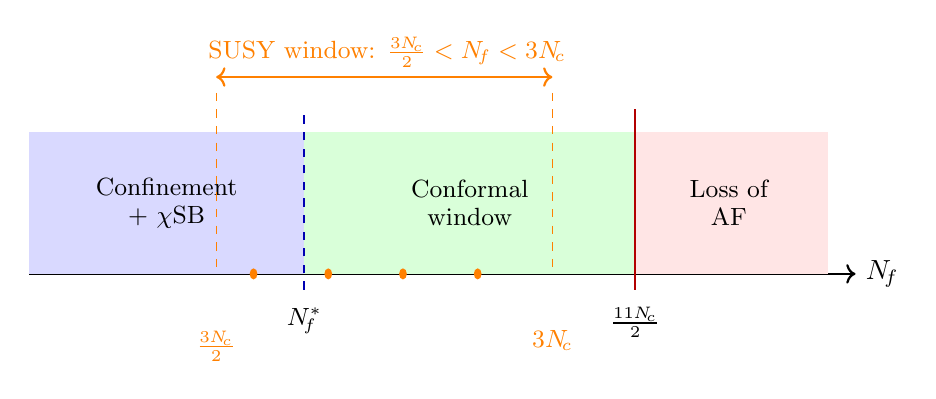
\begin{tikzpicture}[xscale=0.7,yscale=1.0]
  % Axis
  \draw[->,thick] (0,0) -- (15,0) node[right] {$\Nf$};

  % Regions
  \fill[blue!15] (0,0) rectangle (5,1.8);
  \fill[green!15] (5,0) rectangle (11,1.8);
  \fill[red!10] (11,0) rectangle (14.5,1.8);

  % Boundaries
  \draw[thick,dashed,blue!70!black] (5,-0.2) -- (5,2.1);
  \draw[thick,red!70!black] (11,-0.2) -- (11,2.1);

  % Labels for regions
  \node[align=center] at (2.5,0.9) {\small Confinement\\[-2pt]\small $+$ $\chi$SB};
  \node[align=center] at (8,0.9) {\small Conformal\\[-2pt]\small window};
  \node[align=center] at (12.7,0.9) {\small Loss of\\[-2pt]\small AF};

  % Boundary labels
  \node[below] at (5,-0.3) {\small $\Nf^*$};
  \node[below] at (11,-0.3) {\small $\frac{11\Nc}{2}$};

  % SUSY markers (for SU(3))
  \draw[thick,orange,<->] (3.4,2.5) -- (9.5,2.5);
  \node[above,orange] at (6.5,2.5) {\small SUSY window: $\frac{3\Nc}{2} < \Nf < 3\Nc$};
  \draw[orange,dashed] (3.4,2.3) -- (3.4,0);
  \node[below,orange] at (3.4,-0.6) {\small $\frac{3\Nc}{2}$};
  \draw[orange,dashed] (9.5,2.3) -- (9.5,0);
  \node[below,orange] at (9.5,-0.6) {\small $3\Nc$};

  % Tick marks for SU(3) integer values
  \foreach \x in {5,6,7,8} {
    \pgfmathsetmacro{\pos}{3.4 + (\x-4.5)/4.5 * (9.5-3.4)}
    \fill[orange] (\pos,0) circle (2pt);
  }
\end{tikzpicture}
\caption{Phase structure of $\SU{\Nc}$ gauge theory with $\Nf$ fundamental
  Dirac flavours.  The dashed blue line marks the lower boundary of the
  conformal window, $\Nf^*$, which is model-dependent (for non-SUSY theories).
  The solid red line marks the loss of asymptotic freedom at
  $\Nf = 11\Nc/2$.  The orange markers show the SUSY conformal window
  $3\Nc/2 < \Nf < 3\Nc$, which is exact.  For $\SU{3}$, the SUSY conformal
  window contains $\Nf = 5,6,7,8$ (orange dots).}
\label{fig:conformal-window}
\end{figure}

\subsection{\texorpdfstring{$R$}{R}-charge at the conformal fixed point}

In supersymmetric theories (to be developed in Lectures~2--3), the
dimensions of chiral operators at a superconformal fixed point are
determined by their $R$-charges.  The non-anomalous $R$-charge of the
quark superfield is
\begin{equation}
  \Rcharge{Q} = 1 - \frac{\Nc}{\Nf} = \frac{\Nf - \Nc}{\Nf}.
  \label{eq:r-charge}
\end{equation}

The unitarity bound for a chiral operator $\mathcal{O}$ in a superconformal
theory is $\Rcharge{\mathcal{O}} \geq 2/3$ (with saturation corresponding
to a free field).  At the upper edge of the conformal window:
\begin{equation}
  \Nf = 3\Nc: \quad
  \Rcharge{Q} = \frac{3\Nc - \Nc}{3\Nc} = \frac{2}{3}.
  \label{eq:r-charge-upper}
\end{equation}
The unitarity bound is \emph{saturated}: the quarks become free, and the
theory flows to a trivial (free) fixed point.  This is the upper boundary
of the conformal window.

At the lower edge:
\begin{equation}
  \Nf = \frac{3\Nc}{2}: \quad
  \Rcharge{Q} = 1 - \frac{\Nc}{3\Nc/2} = 1 - \frac{2}{3} = \frac{1}{3}.
  \label{eq:r-charge-lower}
\end{equation}
Below this value, the meson operator $M \sim Q\widetilde{Q}$ with
$\Rcharge{M} = 2\Rcharge{Q} < 2/3$ falls below the unitarity bound,
signalling that the conformal description breaks down and confinement sets
in.

\textit{Check:} For $\SU{3}$, $\Nf = 9$: $\Rcharge{Q} = (9-3)/9 = 2/3$.
This is the upper edge; the SUSY conformal window is $4.5 < \Nf < 9$.
$\checkmark$

\begin{exercise}
  Compute $\alphas^*$ at the Banks--Zaks fixed point (two-loop) for
  $\SU{3}$ with $\Nf = 12, 14, 16$.  For which values is the
  perturbative result $\alphas^* \ll 1$ reliable?  Compare with the
  SUSY conformal window prediction for $\SU{3}$.
  \textit{(Exercise Set~2, Problem~2.1.)}
\end{exercise}

\begin{exercise}
  Show that the one-loop SUSY beta function coefficient is
  $\bzero^{\text{SUSY}} = 3\Nc - \Nf$ for $\SU{\Nc}$ with $\Nf$ chiral
  pairs.  Verify that asymptotic freedom requires $\Nf < 3\Nc$.
  \textit{(Exercise Set~2, Problem~2.2.  The derivation will use the NSVZ
  beta function introduced in Lecture~2.)}
\end{exercise}


%% ========================================================================
%%  SECTION 8: Summary and preview
%% ========================================================================
\section{Summary and preview of Lecture~2}
\label{sec:summary}

\subsection{What we have established}

In this lecture, we have introduced the two foundational tools for the
dualised Standard Model programme:

\begin{enumerate}
  \item \textbf{'t~Hooft anomaly matching} (\S\ref{sec:thooft}--\S\ref{sec:general-anomaly}):
    For every exact global symmetry, the anomaly coefficient
    $\mathcal{A}^{abc} = \sum \Tr[T^a\{T^b,T^c\}]$ must be equal when
    computed using \UV{} and \IR{} degrees of freedom.  This is exact
    (Adler--Bardeen) and provides powerful constraints on the
    low-energy spectrum of confining gauge theories.
    \begin{itemize}
      \item This is distinct from gauge anomaly cancellation (which requires
        the anomaly to \emph{vanish}, not merely match).
      \item The warm-up ($\SU{3}$, $\Nf = 2$) illustrated both the
        power and the subtlety of anomaly matching.
      \item The six independent anomaly coefficients for $\SU{\Nc}$ with
        $\Nf$ flavours are tabulated and ready for use.
    \end{itemize}

  \item \textbf{The conformal window} (\S\ref{sec:conformal}):
    $\SU{\Nc}$ with $\Nf$ fundamental flavours exhibits three phases:
    confinement ($\Nf < \Nf^*$), conformal window
    ($\Nf^* < \Nf < 11\Nc/2$), and loss of asymptotic freedom
    ($\Nf > 11\Nc/2$).  The SUSY conformal window is exact:
    $3\Nc/2 < \Nf < 3\Nc$.
\end{enumerate}

\subsection{Preview: Lecture 2}

In Lecture~2, we introduce minimal $\mathcal{N}=1$ supersymmetry:
superfields, the superpotential, $F$- and $D$-term conditions, and the
holomorphic non-renormalisation theorem.  The goal is to access the exact
results (NSVZ beta function, Seiberg duality) that make the dualised
Standard Model programme possible.  No prior SUSY knowledge is assumed.

\subsection{Exercises}

The following exercises develop the material of this lecture:
\begin{itemize}
  \item \textbf{Exercise Set~1} (Anomaly matching):
    \begin{itemize}
      \item[1.1] Verify the six \UV{} anomaly coefficients for
        $\SU{\Nc}$ with $\Nf$ flavours (Table in \S\ref{sec:general-anomaly}).
      \item[1.2] For $\SU{3}$ with $\Nf = 3$, propose an \IR{} baryon
        spectrum and check anomaly matching.
      \item[1.3] Show that for $\Nf = \Nc$, there exists a unique
        baryon that can match all anomalies.
    \end{itemize}
  \item \textbf{Exercise Set~2} (Conformal window):
    \begin{itemize}
      \item[2.1] Compute the Banks--Zaks fixed-point coupling for
        $\SU{3}$ with $\Nf = 12, 14, 16$.
      \item[2.2] Derive $\bzero^{\text{SUSY}} = 3\Nc - \Nf$ from the
        matter content of $\mathcal{N}=1$ SQCD (using the NSVZ beta
        function from Lecture~2).
      \item[2.3] For $\SU{5}$, determine the SUSY conformal window and
        list the integer values of $\Nf$.
    \end{itemize}
\end{itemize}


%% ========================================================================
%%  BIBLIOGRAPHY
%% ========================================================================
\newpage
\begin{thebibliography}{99}

\bibitem{Sannino2024}
  G.~Cacciapaglia and F.~Sannino,
  ``The Standard Model as a Dual Gauge Theory,''
  arXiv:2407.17281 [hep-ph] (2024).

\bibitem{Seiberg1995}
  N.~Seiberg,
  ``Electric--magnetic duality in supersymmetric non-Abelian gauge theories,''
  Nucl.\ Phys.\ \textbf{B435}, 129 (1995)
  [hep-th/9411149].

\bibitem{PS1995}
  M.~E.~Peskin and D.~V.~Schroeder,
  \textit{An Introduction to Quantum Field Theory}
  (Westview Press, 1995).

\bibitem{PeskinTASI1996}
  M.~E.~Peskin,
  ``Duality in Supersymmetric Yang--Mills Theory,''
  TASI 1996 lectures,
  hep-th/9702094.

\bibitem{tHooft1980}
  G.~'t~Hooft,
  ``Naturalness, Chiral Symmetry, and Spontaneous Chiral Symmetry Breaking,''
  in \textit{Recent Developments in Gauge Theories} (Plenum, 1980),
  NATO ASI Series B, Vol.~59.

\bibitem{Adler1969}
  S.~L.~Adler,
  ``Axial-Vector Vertex in Spinor Electrodynamics,''
  Phys.\ Rev.\ \textbf{177}, 2426 (1969).

\bibitem{BellJackiw1969}
  J.~S.~Bell and R.~Jackiw,
  ``A PCAC puzzle: $\pi^0 \to \gamma\gamma$ in the $\sigma$-model,''
  Nuovo Cim.\ \textbf{A60}, 47 (1969).

\bibitem{AdlerBardeen1969}
  S.~L.~Adler and W.~A.~Bardeen,
  ``Absence of Higher-Order Corrections in the Anomalous Axial-Vector
  Divergence Equation,''
  Phys.\ Rev.\ \textbf{182}, 1517 (1969).

\bibitem{BanksZaks1982}
  T.~Banks and A.~Zaks,
  ``On the Phase Structure of Vector-Like Gauge Theories with Massless
  Fermions,''
  Nucl.\ Phys.\ \textbf{B196}, 189 (1982).

\bibitem{WessZumino1971}
  J.~Wess and B.~Zumino,
  ``Consequences of Anomalous Ward Identities,''
  Phys.\ Lett.\ \textbf{B37}, 95 (1971).

\bibitem{Witten1983}
  E.~Witten,
  ``Global Aspects of Current Algebra,''
  Nucl.\ Phys.\ \textbf{B223}, 422 (1983).

\bibitem{ChanTsou1999}
  H.-M.~Chan and S.~T.~Tsou,
  ``The Dualized Standard Model and its Applications --- an Interim Report,''
  hep-ph/9904406 (1999).

\bibitem{Tsou2001}
  S.~T.~Tsou,
  ``Electric--Magnetic Duality and the Dualized Standard Model,''
  hep-th/0110256 (2001).

\bibitem{IntriligatorSeiberg1995}
  K.~Intriligator and N.~Seiberg,
  ``Lectures on Supersymmetric Gauge Theories and Electric--Magnetic
  Duality,''
  Nucl.\ Phys.\ Proc.\ Suppl.\ \textbf{45BC}, 1 (1996)
  [hep-th/9509066].

\bibitem{Bilal2008}
  A.~Bilal,
  ``Lectures on Anomalies,''
  arXiv:0802.0634 [hep-th] (2008).

\bibitem{Terning2002}
  J.~Terning,
  ``TASI-2002 Lectures: Non-perturbative Supersymmetry,''
  hep-th/0306119 (2003).

\bibitem{DeGrand2015}
  T.~DeGrand,
  ``Lattice tests of beyond Standard Model dynamics,''
  Rev.\ Mod.\ Phys.\ \textbf{88}, 015001 (2016).

\bibitem{Hasenbusch2021}
  A.~Hasenfratz \textit{et al.},
  ``Infrared fixed point of the $\SU{3}$ gauge theory with $\Nf=10$
  flavors,''
  Phys.\ Rev.\ \textbf{D104}, 074509 (2021).

\bibitem{Caswell1974}
  W.~E.~Caswell,
  ``Asymptotic Behavior of Non-Abelian Gauge Theories to Two-Loop Order,''
  Phys.\ Rev.\ Lett.\ \textbf{33}, 244 (1974).

\end{thebibliography}

\end{document}
